\documentclass[fleqn, a4paper, 11pt, oneside]{amsart}
%\usepackage[top = 2cm, bottom = 1cm, left = 1cm, right = 1cm]{geometry}
\usepackage{exsheets, tasks}
\usepackage{amsmath, amssymb, amsthm} %standard AMS packages
\usepackage{marginnote} %marginnotes
\usepackage{gensymb} %miscellaneous symbols
\usepackage{commath} %differential symbols
\usepackage{xcolor} %colours
\usepackage{cancel} %cancelling terms
\usepackage[free-standing-units, space-before-unit]{siunitx} %formatting units
	\sisetup
	{
		per-mode=fraction,
		fraction-function=\frac
	}
\usepackage{tikz, pgfplots} %diagrams
\usetikzlibrary{calc, hobby, patterns, intersections, decorations.markings}
\usepackage{graphicx} %inserting graphics
\usepackage{hyperref} %hyperlinks
\usepackage{datetime} %date and time
\usepackage{ulem} %underline for \emph{}
\usepackage{xfrac} %inline fractions
\usepackage{enumerate,enumitem} %numbered lists
\usepackage{float} %inserting floats
\usepackage{circuitikz}[american voltages, american currents] %circuit diagrams
\usepackage[utf8]{inputenc}
\usepackage{booktabs}
\usepackage{todonotes}

\newcommand\numberthis{\addtocounter{equation}{1}\tag{\theequation}} %adds numbers to specific equations in non-numbered list of equations

\newcommand{\AxisRotator}[1][rotate=0]{
	\tikz [x=0.25cm,y=0.60cm,line width=.2ex,-stealth,#1] \draw (0,0) arc (-150:150:1 and 1);%
} %rotation symbols on axes

\theoremstyle{definition}
\newtheorem{example}{Example}
\newtheorem{definition}{Definition}

\theoremstyle{theorem}
\newtheorem{theorem}{Theorem}

\newcommand{\curl}{\mathrm{curl\,}}

\makeatletter
\@addtoreset{section}{part} %resets section numbers in new part
\makeatother

\renewcommand{\thesubsection}{(\arabic{subsection})}
\renewcommand{\thesection}{(\arabic{section})}

\renewcommand{\emph}{\uline}

\renewcommand{\tilde}{\widetilde}

%section headings on left
\makeatletter
\def\specialsection{\@startsection{section}{1}%
	\z@{\linespacing\@plus\linespacing}{.5\linespacing}%
	%  {\normalfont\centering}}% DELETED
	{\normalfont}}% NEW
\def\section{\@startsection{section}{1}%
	\z@{.7\linespacing\@plus\linespacing}{.5\linespacing}%
	%  {\normalfont\scshape\centering}}% DELETED
	{\normalfont\scshape}}% NEW
\makeatother

%forces newline after subsection
\makeatletter
\def\subsection{\@startsection{subsection}{3}%
	\z@{.5\linespacing\@plus.7\linespacing}{.1\linespacing}%
	{\normalfont\itshape}}
\makeatother

\settasks{counter-format = tsk[1].}

\SetupExSheets{solution/print = true}

%opening
\title{Quantum and Solid State Physics : Assignment 12}
\author
{
	Aakash Jog\\
	ID : 989323563
}
\date{\formatdate{14}{1}{2016}}

\begin{document}

\tikzset{->-/.style={decoration={
  markings,
  mark=at position #1 with {\arrow{>}}},postaction={decorate}}}

\maketitle
%\setlength{\mathindent}{0pt}

\begin{question}
	A semiconductor is under constant illumination through a narrow opening.
	The illumination generates EHPs in the volume below the illuminated area.
	Given that in this semiconductor the diffusion coefficient of holes is larger than the diffusion coefficient of electrons, what will be the direction of the internal electric field at steady state?
\end{question}

\begin{solution}
	As the diffusion coefficient of holes is larger than the diffusion coefficient of electrons, the mobility of holes is also larger than the mobility of electrons.
	Therefore, the holes diffuse more easily than the electrons.
	Hence, the curve of $\hat{p}(x)$ with respect to $x$, is wider than that of $\hat{n}(x)$.\\
	Therefore, the internal electric field is \emph{directed inwards, towards the centre}.
\end{solution}

\begin{question}
	A silicon sample at equilibrium and at room temperature is doped N-type with a doping concentration profile as shown.
	\begin{figure}[H]
		\centering
		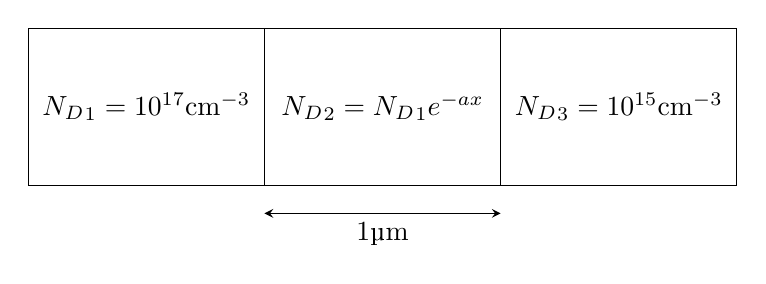
\begin{tikzpicture}
			\def\l{3};
			\def\h{2};

			\begin{scope}
				\draw (0,0) rectangle (\l,\h);
				\node at (\l/2,\h/2) {${N_D}_1 = 10^{17} \si{\per\centi\metre\cubed}$};
			\end{scope}

			\begin{scope}[xshift = \l cm]
				\draw (0,0) rectangle (\l,\h);
				\node at (\l/2,\h/2) {${N_D}_2 = {N_D}_1 e^{-a x}$};
				\draw[stealth-stealth, yshift = -10] (0,0) -- (\l,0) node [midway, below] {$1 \si{\micro\metre}$};
			\end{scope}

			\begin{scope}[xshift = 2*\l cm]
				\draw (0,0) rectangle (\l,\h);
				\node at (\l/2,\h/2) {${N_D}_3 = 10^{15} \si{\per\centi\metre\cubed}$};
			\end{scope}
		\end{tikzpicture}
	\end{figure}
	\begin{enumerate}
		\item
			Calculate the electric field $\overrightarrow{E}(x)$ in \si{\volt\per\centi\metre} in all three regions and plot $\overrightarrow{E}(x)$ with respect to $x$, across the entire sample.
		\item
			After calculating the electric field $\overrightarrow{E}(x)$ in all three regions, we expect to obtain an energy band diagram as shown.
			\begin{figure}[H]
				\centering
				\begin{tikzpicture}
					\def\l{3};
					\def\eConduction{3};
					\def\eIntrinsic{2};
					\def\eValence{1};

					\begin{scope}
						\draw (0,\eValence) node [left] {$E_V$} -- (\l,\eValence);
						\draw[dashed] (0,\eIntrinsic) node [left] {$E_i$} -- (\l,\eIntrinsic);
						\draw (0,\eConduction) node [left] {$E_C$} -- (\l,\eConduction);
					\end{scope}

					\begin{scope}
						\draw (\l,\eValence) -- (2*\l,\eValence + 1);
						\draw[dashed] (\l,\eIntrinsic) -- (2*\l,\eIntrinsic + 1);
						\draw (\l,\eConduction) -- (2*\l,\eConduction + 1);
					\end{scope}

					\begin{scope}
						\draw (2*\l,\eValence + 1) -- (3*\l,\eValence + 1);
						\draw[dashed] (2*\l,\eIntrinsic + 1) -- (3*\l,\eIntrinsic + 1);
						\draw (2*\l,\eConduction + 1) -- (3*\l,\eConduction + 1);
					\end{scope}
				\end{tikzpicture}
			\end{figure}
			Draw the built-in voltage $V_{B I}$ in the sample.
	\end{enumerate}
\end{question}

\begin{solution}
	\begin{enumerate}
		\item
			As the concentration profile is continuous at the interface of regions 2 and 3,
			\begin{align*}
				10^{17} e^{-a 10^{-6}}    & = 10^{15}                   \\
				\therefore e^{-a 10^{-6}} & = 10^{-2}                   \\
				\therefore -a 10^{-6}     & = \ln\left( 10^{-2} \right) \\
                                                          & = -2 \ln(10)                \\
				\therefore a              & = 2 \ln(10) 10^6            \\
                                                          & = 4.6 \times 10^6
			\end{align*}
			Therefore,
			\begin{align*}
				\overrightarrow{E}_1(x) & = -\frac{k T}{q} \frac{1}{{N_D}_1}(x) \dod{N_d(x)}{x} \\
                                                        & = -\frac{k T}{q} \frac{1}{10^{17}} 0                  \\
                                                        & = 0
			\end{align*}
			Therefore,
			\begin{align*}
				\overrightarrow{E}_2(x) & = -\frac{k T}{q} \frac{1}{{N_D}_2}(x) \dod{N_d(x)}{x}                                 \\
                                                        & = -\frac{k T}{q} \frac{1}{10^{17} e^{-a x}} \dod{10^{17} e^{-a x}}{x}                 \\
                                                        & = -\frac{k T}{q} \frac{1}{10^{17} e^{-a x}} \left( -a \times 10^{17} e^{-a x} \right) \\
                                                        & = \frac{k T}{q} a
			\end{align*}
			Therefore,
			\begin{align*}
				\overrightarrow{E}_3(x) & = -\frac{k T}{q} \frac{1}{{N_D}_3}(x) \dod{N_d(x)}{x} \\
                                                        & = -\frac{k T}{q} \frac{1}{10^{15}} 0                  \\
                                                        & = 0
			\end{align*}
		\item
			~\\
			\begin{figure}[H]
				\centering
				\begin{tikzpicture}
					\def\l{3};
					\def\eConduction{3};
					\def\eIntrinsic{2};
					\def\eValence{1};

					\begin{scope}
						\draw (0,\eValence) node [left] {$E_V$} -- (\l,\eValence);
						\draw[dashed] (0,\eIntrinsic) node [left] {$E_i$} -- (\l,\eIntrinsic);
						\draw (0,\eConduction) node [left] {$E_C$} -- (\l,\eConduction);
					\end{scope}

					\begin{scope}
						\draw (\l,\eValence) -- (2*\l,\eValence + 1);
						\draw[dashed] (\l,\eIntrinsic) -- (2*\l,\eIntrinsic + 1);
						\draw (\l,\eConduction) -- (2*\l,\eConduction + 1);
					\end{scope}

					\begin{scope}
						\draw (2*\l,\eValence + 1) -- (3*\l,\eValence + 1);
						\draw[dashed] (2*\l,\eIntrinsic + 1) -- (3*\l,\eIntrinsic + 1);
						\draw (2*\l,\eConduction + 1) -- (3*\l,\eConduction + 1);
					\end{scope}

					\begin{scope}[stealth-stealth]
						\draw (\l/2,\eConduction) -- (\l/2,\eConduction + 1) node [midway,left] {$q V_{B I}$};
					\end{scope}
				\end{tikzpicture}
			\end{figure}
	\end{enumerate}
\end{solution}

\end{document}
